\documentclass{article}
\usepackage[marginparsep=8pt, margin=1.75cm, top=2.5cm, bottom=2.5cm]{geometry}
\usepackage[english]{babel}
\usepackage{listings}
\usepackage[siunitx]{circuitikz}
\usepackage{booktabs}
\usepackage{siunitx}
\usepackage{graphicx} % Required for inserting images
\usepackage{amsmath}
\usepackage{amssymb}
\usepackage{siunitx} % for v pr sqrt htz
\usepackage{pgfplots}
\usepackage{tikz}
\usepackage{tikz-3dplot}
\usepackage{subcaption}
\usepackage[
backend=biber,
style=numeric,
sorting=none
]{biblatex}

%curtom macro
\newcommand{\VperRootHz}[1]{\frac{\mathrm{#1V}}{\sqrt{\mathrm{Hz}}}}  %use $VperRootHz{n}$, $VperRootHz{\mu}$ etc

\pgfplotsset{compat=newest}





\begin{document}

% \input{forside.tex}
\begin{figure}
    \centering
    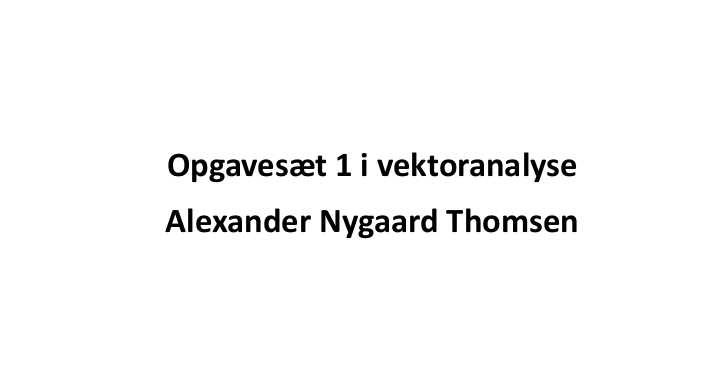
\includegraphics{forside_ting.png}
\end{figure}
\clearpage
% \section{Exercise 1}
\textit{consider the cube $C = {(x,y,z) \in \mathbb{R}^3 | 
0 \leq x \leq 1,
0 \leq y \leq 1,
0 \leq z \leq 1}$ in $\mathbb{R}^3$. 
Find the angle between the plane $P_1$ containing
the 3 points: $(0,1,0),(1,0,0),(1,1,1)$ and the plane $P_2$ 
containing the 3 points: $(0,0,0),(1,1,0),(1,0,1)$.}

\tdplotsetmaincoords{70}{120}

\begin{tikzpicture}[tdplot_main_coords, scale=2]
    
%cube coordinates
\coordinate (O) at (0,0,0);
\coordinate (X) at (1,0,0);
\coordinate (Y) at (0,1,0);
\coordinate (Z) at (0,0,1);

%plane1
\coordinate (P1A) at (0,1,0); 
\coordinate (P1B) at (1,0,0);
\coordinate (P1C) at (1,1,1);
%plane2
\coordinate (P2A) at (0,0,0); 
\coordinate (P2B) at (1,1,0);
\coordinate (P2C) at (1,0,1);


\coordinate (XY) at (1,1,0);
\coordinate (XZ) at (1,0,1);
\coordinate (YZ) at (0,1,1);
\coordinate (XYZ) at (1,1,1);

%edges
\draw (O) -- (X) -- (XY) -- (Y) -- cycle;
\draw (Z) -- (XZ) -- (XYZ) -- (YZ) -- cycle;
\draw (O) -- (Z);
\draw (X) -- (XZ);
\draw (Y) -- (YZ);
\draw (XY) -- (XYZ);


%plane throught the three corners
% \filldraw[fill=blue!30, opacity=0.6, draw=blue, thick]
%     (A) -- (B) -- (C) -- cycle;
%plane p1
\filldraw[fill=blue!30, opacity=0.6, draw=blue, thick]
    (P1A) -- (P1B) -- (P1C) -- cycle;
%plane p2
\filldraw[fill=red!30, opacity=0.6, draw=red, thick]
    (P2A) -- (P2B) -- (P2C) -- cycle;


%mark corners
\fill (X) circle (1pt) node[below] {$X$};
\fill (Y) circle (1pt) node[left] {$Y$};
\fill (Z) circle (1pt) node[above] {$Z$};


\end{tikzpicture}

To find the angle between the two planes, we must firstly find the normal vector that
the individual planes define and then find the angle between those two.

\[
\vec{P_{1X}} =
\begin{pmatrix}
0 \\ 1 \\ 0
\end{pmatrix},
\qquad
\vec{P_{1Y}} =
\begin{pmatrix}
1 \\ 0 \\ 0
\end{pmatrix},
\qquad
\vec{P_{1Z}} =
\begin{pmatrix}
1 \\ 1 \\ 1
\end{pmatrix}
\]\\

Vectors for $P_1$
\[
\vec{P_{1XY}} = \vec{P_{1X}} - \vec{P_{1Y}} = 
\begin{pmatrix}
0 - 1 \\ 1 - 0 \\ 0 - 0    
\end{pmatrix} 
= 
\begin{pmatrix}
-1 \\ 1 \\ 0
\end{pmatrix},
\qquad
\vec{P_{1XZ}} = \vec{P_{1X}} - \vec{P_{1Z}} = 
\begin{pmatrix}
0 - 1 \\ 1 - 1 \\ 0 - 1    
\end{pmatrix} 
=
\begin{pmatrix}
-1\\0\\-1
\end{pmatrix}
\]

The normal vector for plane $P1$ is the cross product of the two vectors in the plane.
\[
\vec{N1} =
\vec{P_{1XY}} \times \vec{P_{1XZ}}
=
\begin{pmatrix}
-1\\-1\\1
\end{pmatrix}
\]
The procedure goes for the second set of points, to generate the set of vectors, the plane they sit on, and the 
normal vector that extends from it.

%P2
Points
\[
\vec{P_{2X}} =
\begin{pmatrix}
0 \\ 0 \\ 0
\end{pmatrix},
\qquad
\vec{P_{2Y}} =
\begin{pmatrix}
1 \\ 1 \\ 0
\end{pmatrix},
\qquad
\vec{P_{2Z}} =
\begin{pmatrix}
1 \\ 0 \\ 1
\end{pmatrix}
\]
Vectors for $P2$
\[
\vec{P_{2XY}} = \vec{P_{2X}} - \vec{P_{2Y}} = 
\begin{pmatrix}
0 - 1 \\ 0 - 1 \\ 0 - 0    
\end{pmatrix} 
= 
\begin{pmatrix}
-1 \\ -1 \\ 0
\end{pmatrix},
\qquad
\vec{P_{2XZ}} = \vec{P_{2X}} - \vec{P_{2Z}} = 
\begin{pmatrix}
0 - 1 \\ 0 - 0 \\ 0 - 1    
\end{pmatrix} 
=
\begin{pmatrix}
-1\\0\\-1
\end{pmatrix}
\]
Normal vector from plane $P2$
\[
\vec{N2} =
\vec{P_{2XY}} \times \vec{P_{2XZ}}
=
\begin{pmatrix}
1\\-1\\-1
\end{pmatrix}
\]

The angle between these two vectors will then indicate the angle between the planes $P1$ and $P2$
\[
    \theta = cos^{-1}(\frac{N1 \cdot N2}{|N1||N2|}) \Rightarrow 
    \frac{(-1)(1)+(-1)(-1)+(1)(-1)}{\sqrt{(-1)^2(-1)^2(1)^2}\cdot \sqrt{(1)^2(-1)^2(-1)^2}} \Rightarrow 
    \frac{-1}{\sqrt{(3)^2}} \rightarrow = cos^{-1}(\frac{-1}{3}) * \frac{180}{\pi} \approx 109.492
\]



% \clearpage
% \section{exercise 2}
\textit{Find the center of mass ($\bar{x},\bar{y},\bar{z}$), for the wire C shaped as a helix, with density p = kz, (k is a constant).
The wire C has parametrization:}
\[
x(t) = 3cos(t), y(t)=3sin(t), z(t)=4t, 0\leq t \leq \pi
\]

\textit{The following equations define the center of mass:}
\begin{itemize}
    \item The curve length $s(t)$, as a function of t satisfies: $\frac{ds}{dt} = \sqrt{x'(t)^2 + y'(t)^2 + z'(t)^2}$
    \item $m = \int_c p(x,y,z)ds$
    \item $\bar{x} = \frac{1}{m} \int_c xp(x,y,z)ds, \bar{y} = \frac{1}{m}\int_c yp(x,y,z)ds, \bar{z}=\frac{1}{m}\int_c zp(x,y,z)ds$ 
\end{itemize}

This is a rather convoluted question, essentially asking, if we have a piece of wire, in this case a 
helix, meaning there is a one large curve, since it is bounded to $0\leq t \leq \pi$, what is the 
position in space of the center of its mass. The parametrization describes how the \textit{coil} will 
expand if we increase to. The first two components $x$ and $y$ are trigonometric functions, causing the
direction to be circular around the $z$-axis, and the $z$ component simply indicates that it increases
linearly with $t$.\\

Firstly we need to calculate the change in $t$ into changes on the actual physical wire. We're given the
density $p$ and mass is the product of density and lenght. So the curve length is calculated as:


\[\frac{ds}{dt} = \sqrt{x'(t)^2 + y'(t)^2 + z'(t)^2}\] 
differentiating the functions
\[x'(t) = \frac{d}{dt}x(t) \Rightarrow -3sin(t)\]
\[y'(t) = \frac{d}{dt}y(t) = \frac{d}{dt}3cos(t)\]
\[z'(t) = \frac{d}{dt}z(t) = \frac{d}{dt}t(t)\]
into the curve length
\[\frac{ds}{dt} = \sqrt{(-3\cdot sin(t))^2+(3\cdot cos(t))^2+(4)^2}\]
rearrange, use distributive property and recognize the idiot formula $sin^2(t) + cos^2(t) = 1$
\[=\sqrt{9 + 1 + 16}  = \sqrt{25} = 5\]
\[ ds = 5dt\]
Relationship for density is given, with z given and k is some constant, it can we rewritten as:
\[p = k \cdot z \]
\[p = 4tk\]
Substituted into the mass relationship, with a change of variable from the $\frac{ds}{dt}$ relationship,
so that mass is now in terms of $t$:
\[m = \int_0^\pi (4tk)(5)dt \Rightarrow 10k\pi^2\]
Since the lower bound is zero and are a single term with factors, it gets reduced to zero.
Each of the coordinates for the center of mass can now be evaluated.
\[\bar{x} = \frac{1}{10k\pi^2}\int_0^\pi 3\cdot cos(t)\cdot 4t \cdot k \cdot 5 dt\]
\[ = \frac{60k}{10k\pi^2} \int_0^\pi t\cdot cos(t)dt \Rightarrow  \frac{60k}{10k\pi^2} [t\cdot sin(t) +cos(t)]_0^\pi\]
\[= \frac{6}{\pi^2} \cdot (-1) - \frac{6}{\pi^2}+cos(0)=-\frac{12}{\pi^2}\]
The same can be done for the two other coordinates:
\[\bar{y} = \frac{1}{10k\pi^2}\int_0^\pi 3\cdot sin(t)\cdot 4t \cdot k \cdot 5 dt\]
\[ = \frac{60k}{10k\pi^2} \int_0^\pi t \cdot sin(t)dt \Rightarrow 
\frac{6}{\pi^2}[sin(t) - t\cdot cos(t)]_0^\pi \Rightarrow \frac{6}{\pi}\]

\[\bar{z} = \frac{1}{10k\pi^2}\int_0^\pi (4t)\cdot 4t \cdot k \cdot 5 dt\]
\[ = \frac{80k}{10k\pi^2} \int_0^\pi t^2 dt \Rightarrow 
\frac{8}{\pi^2}[\frac{t^3}{2}]_0^\pi \Rightarrow \frac{8\pi}{3}\]

Giving coordinates:
\[[\bar{x}, \bar{y}, \bar{z}] = [-\frac{12}{\pi^2}, \frac{6}{\pi}, \frac{8\pi}{3} ]\]




% \clearpage
% \section{exercise 3}
\textit{Let $F$ be a vector field on $\mathbb{R}^3$ given by:}
\[F(x,y,z) = (0,0,1)\]
\textit{Using surface integrals, show that the flux through the upper hemisphere of the unit sphere:}
\[S_{+}^2 = \{(x,y,z)\in \mathbb{R}^3  |x^2+y^2+z^2 = 1, z \geq 0\}\] 
\textit{is the same as the flux through the unit disk in the xy-plane}
\[D = \{(x,y,z)\in \mathbb{R}^3 |x^2+y^2 \leq 1, z=0\}\]\\

\subsection{the unit sphere}
we're given a vector field that essentially shows an upwards flow in
in the $Z$ direction, with a magnitude of 1. 
\[F(x,y,z) = (0,0,1)\]
As for the hemisphere we're bounded for $ z\geq0$, therefore
we can solve the hemisphere equation for z, essentially telling us
the height $z$ at any point in the sphere over $(x,y)$ on the disc underneath.

\[x^2+y^2+z^2 = 1 \Rightarrow z = \sqrt{1-x^2-y^2}\]
this can be parameterized using x and y 
\[r(x,y) = (x,y,\sqrt{1-x^2-y^2})\]
and x and y must lie within the unit disc
\[x^2+y^2 = 1\]

We can then differentiate r with respect to x 
\[r_x = \frac{\delta r}{\delta x} \Rightarrow r_x = (1,0, \frac{-x}{\sqrt{1-x^2-y^2}})\]
and r with respect y
\[r_y = \frac{\delta r}{\delta x} \Rightarrow r_x = (0,1, \frac{-y}{\sqrt{1-x^2-y^2}})\]
This lets us find the vector surface element $\textbf{n}ds$, this is done by creaing the
vector cross product 
\[ (r_x \times r_y) = (\frac{x}{\sqrt{1-x^2-y^2}},\frac{y}{\sqrt{1-x^2-y^2}},1 )\]

this leads to the expression 
\[\textbf{n}dS = (r_x \times r_y) = (\frac{x}{\sqrt{1-x^2-y^2}},\frac{y}{\sqrt{1-x^2-y^2}},1 ) dx dy\]

This can be dottet with our vector field:
\[\textbf{F} \cdot \textbf{n} dS = (0,0,1) \cdot (\frac{x}{\sqrt{1-x^2-y^2}},\frac{y}{\sqrt{1-x^2-y^2}},1 ) dx dy \]
which evaluates to 
\[= 1 dx dy\]

Now we can find the surface integral over the surface S, by using the vector field.
\[Q_s = \iint_S \textbf{F} \cdot \textbf{n} dS\]
The limits here can be derived:
\[x^2+y^2 = 1 \Rightarrow x = \pm \sqrt{1-y^2}\]
therefore y is bound within.
\[-1\leq y \leq1\]
and x is bound by
\[-\sqrt{1-y^2} \leq x \leq \sqrt{1-y^2}\]
Inserting these limits into the integral
\[Q_s = \int_{-1}^{1}\int_{-\sqrt{1-y^2}}^{\sqrt{1-y^2}} 1 dx dy\]
These have been solved using MATHCAD
The inner integration 
\[\int_{-\sqrt{1-y^2}}^{\sqrt{1-y^2}} 1 dx = 2\sqrt{1-y^2}\]
And the outer aswell
\[\int_{-1}^{1}2\sqrt{1-y^2} dy = \pi \] 

\subsection{the unit disk}
To calculate the flux through the disk, the same field $F = (0,0,1)$, we need the normal vector to the surface of the disk in the
same orientation as the vector field meaning $\hat{\textbf{n} = (0,0,1)}$\\
The dot-product of these two vectors can be expressed as 
\[ \textbf{F} \cdot \textbf{n} = (0,0,1) \cdot (0,0,1) = 1\]
this tells us that they point in the same direction
This lets us create the integral of the disk flux.
However we can in this case use the same integral limits as the unit sphere.
This is evaluated using MATHCAD.
\[\iint_D \textbf[F] \cdot \textbf{n} dS = \int_{-1}^{1} \int_{-\sqrt{1-y^2}}^{\sqrt{1-y^2}} 1dxdy = \pi\]

Both methods equates to $\pi$ thus the flux must be the same.

% \clearpage
% \section{exercise 4}
\textit{let $\phi$ be a scalar field and $F$ a vector field given by:}
\[\phi(x,y,z) = xyz^2\] and \[F(x,y,z) = (x^2,y,z)\]

\begin{itemize}
    \item Find $\nabla\phi$ and $\nabla \cdot F$ and $\nabla \cdot (\phi F)$
    \item try to deduce a general expression for $\nabla \cdot (\phi F)$ expressed by $\nabla \phi$ and $\nabla \cdot F$
\end{itemize}

\subsection{opgave 1}
Given the scalar field, the gradient $\nabla$ can be found by differentiating 
once in each direction. The gradient of a scalar field is a vector field.
\[
\nabla \cdot \phi = 
\begin{bmatrix}
\frac{\partial \phi}{\partial x}\\
\frac{\partial \phi}{\partial y}\\
\frac{\partial \phi}{\partial z}
\end{bmatrix}
=
\begin{bmatrix}
{yz^2}\\
{xz^2}\\
{2xyz}
\end{bmatrix}
\]
\subsection{opgave 2}
The next is finding the divergence of a vector field, which turns it into a scalar field.
\[
\nabla \cdot F = 
\frac{\partial F_x}{\partial x} 
+ \frac{\partial F_y}{\partial y} 
+ \frac{\partial F_z}{\partial z}
= 2x + 2
\]
\subsection{opgave 3}
\[\phi \textbf{F} = xyz^2(x^2,y,z)\]
can be expressed as:
\[ \phi \textbf{F} = (x^3yz^2, xy^2, xyz^3)\]
now the divergencecan be taken
\[\nabla \cdot (\phi \textbf{F}) = \frac{\delta}{\delta x}(x^3yz^2)+ \frac{\delta}{\delta y}(xy^2)+\frac{\delta }{\delta z}(xyz^3)\]
individually they become:
\[\frac{\delta}{\delta x}(x^3yz^2) =3x^2yz^2\]
\[\frac{\delta}{\delta x}(xy^2) = 2xyz^2\]
\[\frac{\delta}{\delta x}(xyz^3) = 3xyz^2\]

the final result will be a sum of those terms
I made some mistakes and this is how far i got...
% \section{exercise 2}
\textit{Find the center of mass ($\bar{x},\bar{y},\bar{z}$), for the wire C shaped as a helix, with density p = kz, (k is a constant).
The wire C has parametrization:}
\[
x(t) = 3cos(t), y(t)=3sin(t), z(t)=4t, 0\leq t \leq \pi
\]

\textit{The following equations define the center of mass:}
\begin{itemize}
    \item The curve length $s(t)$, as a function of t satisfies: $\frac{ds}{dt} = \sqrt{x'(t)^2 + y'(t)^2 + z'(t)^2}$
    \item $m = \int_c p(x,y,z)ds$
    \item $\bar{x} = \frac{1}{m} \int_c xp(x,y,z)ds, \bar{y} = \frac{1}{m}\int_c yp(x,y,z)ds, \bar{z}=\frac{1}{m}\int_c zp(x,y,z)ds$ 
\end{itemize}

This is a rather convoluted question, essentially asking, if we have a piece of wire, in this case a 
helix, meaning there is a one large curve, since it is bounded to $0\leq t \leq \pi$, what is the 
position in space of the center of its mass. The parametrization describes how the \textit{coil} will 
expand if we increase to. The first two components $x$ and $y$ are trigonometric functions, causing the
direction to be circular around the $z$-axis, and the $z$ component simply indicates that it increases
linearly with $t$.\\

Firstly we need to calculate the change in $t$ into changes on the actual physical wire. We're given the
density $p$ and mass is the product of density and lenght. So the curve length is calculated as:


\[\frac{ds}{dt} = \sqrt{x'(t)^2 + y'(t)^2 + z'(t)^2}\] 
differentiating the functions
\[x'(t) = \frac{d}{dt}x(t) \Rightarrow -3sin(t)\]
\[y'(t) = \frac{d}{dt}y(t) = \frac{d}{dt}3cos(t)\]
\[z'(t) = \frac{d}{dt}z(t) = \frac{d}{dt}t(t)\]
into the curve length
\[\frac{ds}{dt} = \sqrt{(-3\cdot sin(t))^2+(3\cdot cos(t))^2+(4)^2}\]
rearrange, use distributive property and recognize the idiot formula $sin^2(t) + cos^2(t) = 1$
\[=\sqrt{9 + 1 + 16}  = \sqrt{25} = 5\]
\[ ds = 5dt\]
Relationship for density is given, with z given and k is some constant, it can we rewritten as:
\[p = k \cdot z \]
\[p = 4tk\]
Substituted into the mass relationship, with a change of variable from the $\frac{ds}{dt}$ relationship,
so that mass is now in terms of $t$:
\[m = \int_0^\pi (4tk)(5)dt \Rightarrow 10k\pi^2\]
Since the lower bound is zero and are a single term with factors, it gets reduced to zero.
Each of the coordinates for the center of mass can now be evaluated.
\[\bar{x} = \frac{1}{10k\pi^2}\int_0^\pi 3\cdot cos(t)\cdot 4t \cdot k \cdot 5 dt\]
\[ = \frac{60k}{10k\pi^2} \int_0^\pi t\cdot cos(t)dt \Rightarrow  \frac{60k}{10k\pi^2} [t\cdot sin(t) +cos(t)]_0^\pi\]
\[= \frac{6}{\pi^2} \cdot (-1) - \frac{6}{\pi^2}+cos(0)=-\frac{12}{\pi^2}\]
The same can be done for the two other coordinates:
\[\bar{y} = \frac{1}{10k\pi^2}\int_0^\pi 3\cdot sin(t)\cdot 4t \cdot k \cdot 5 dt\]
\[ = \frac{60k}{10k\pi^2} \int_0^\pi t \cdot sin(t)dt \Rightarrow 
\frac{6}{\pi^2}[sin(t) - t\cdot cos(t)]_0^\pi \Rightarrow \frac{6}{\pi}\]

\[\bar{z} = \frac{1}{10k\pi^2}\int_0^\pi (4t)\cdot 4t \cdot k \cdot 5 dt\]
\[ = \frac{80k}{10k\pi^2} \int_0^\pi t^2 dt \Rightarrow 
\frac{8}{\pi^2}[\frac{t^3}{2}]_0^\pi \Rightarrow \frac{8\pi}{3}\]

Giving coordinates:
\[[\bar{x}, \bar{y}, \bar{z}] = [-\frac{12}{\pi^2}, \frac{6}{\pi}, \frac{8\pi}{3} ]\]




% \section{exercise 3}
\textit{Let $F$ be a vector field on $\mathbb{R}^3$ given by:}
\[F(x,y,z) = (0,0,1)\]
\textit{Using surface integrals, show that the flux through the upper hemisphere of the unit sphere:}
\[S_{+}^2 = \{(x,y,z)\in \mathbb{R}^3  |x^2+y^2+z^2 = 1, z \geq 0\}\] 
\textit{is the same as the flux through the unit disk in the xy-plane}
\[D = \{(x,y,z)\in \mathbb{R}^3 |x^2+y^2 \leq 1, z=0\}\]\\

\subsection{the unit sphere}
we're given a vector field that essentially shows an upwards flow in
in the $Z$ direction, with a magnitude of 1. 
\[F(x,y,z) = (0,0,1)\]
As for the hemisphere we're bounded for $ z\geq0$, therefore
we can solve the hemisphere equation for z, essentially telling us
the height $z$ at any point in the sphere over $(x,y)$ on the disc underneath.

\[x^2+y^2+z^2 = 1 \Rightarrow z = \sqrt{1-x^2-y^2}\]
this can be parameterized using x and y 
\[r(x,y) = (x,y,\sqrt{1-x^2-y^2})\]
and x and y must lie within the unit disc
\[x^2+y^2 = 1\]

We can then differentiate r with respect to x 
\[r_x = \frac{\delta r}{\delta x} \Rightarrow r_x = (1,0, \frac{-x}{\sqrt{1-x^2-y^2}})\]
and r with respect y
\[r_y = \frac{\delta r}{\delta x} \Rightarrow r_x = (0,1, \frac{-y}{\sqrt{1-x^2-y^2}})\]
This lets us find the vector surface element $\textbf{n}ds$, this is done by creaing the
vector cross product 
\[ (r_x \times r_y) = (\frac{x}{\sqrt{1-x^2-y^2}},\frac{y}{\sqrt{1-x^2-y^2}},1 )\]

this leads to the expression 
\[\textbf{n}dS = (r_x \times r_y) = (\frac{x}{\sqrt{1-x^2-y^2}},\frac{y}{\sqrt{1-x^2-y^2}},1 ) dx dy\]

This can be dottet with our vector field:
\[\textbf{F} \cdot \textbf{n} dS = (0,0,1) \cdot (\frac{x}{\sqrt{1-x^2-y^2}},\frac{y}{\sqrt{1-x^2-y^2}},1 ) dx dy \]
which evaluates to 
\[= 1 dx dy\]

Now we can find the surface integral over the surface S, by using the vector field.
\[Q_s = \iint_S \textbf{F} \cdot \textbf{n} dS\]
The limits here can be derived:
\[x^2+y^2 = 1 \Rightarrow x = \pm \sqrt{1-y^2}\]
therefore y is bound within.
\[-1\leq y \leq1\]
and x is bound by
\[-\sqrt{1-y^2} \leq x \leq \sqrt{1-y^2}\]
Inserting these limits into the integral
\[Q_s = \int_{-1}^{1}\int_{-\sqrt{1-y^2}}^{\sqrt{1-y^2}} 1 dx dy\]
These have been solved using MATHCAD
The inner integration 
\[\int_{-\sqrt{1-y^2}}^{\sqrt{1-y^2}} 1 dx = 2\sqrt{1-y^2}\]
And the outer aswell
\[\int_{-1}^{1}2\sqrt{1-y^2} dy = \pi \] 

\subsection{the unit disk}
To calculate the flux through the disk, the same field $F = (0,0,1)$, we need the normal vector to the surface of the disk in the
same orientation as the vector field meaning $\hat{\textbf{n} = (0,0,1)}$\\
The dot-product of these two vectors can be expressed as 
\[ \textbf{F} \cdot \textbf{n} = (0,0,1) \cdot (0,0,1) = 1\]
this tells us that they point in the same direction
This lets us create the integral of the disk flux.
However we can in this case use the same integral limits as the unit sphere.
This is evaluated using MATHCAD.
\[\iint_D \textbf[F] \cdot \textbf{n} dS = \int_{-1}^{1} \int_{-\sqrt{1-y^2}}^{\sqrt{1-y^2}} 1dxdy = \pi\]

Both methods equates to $\pi$ thus the flux must be the same.


%aflevering 2
\section{Exercise 1}
\textit{Let $F$ be a vector field on $\mathbb{R}^3$ given by:}
\[F(x,y,z)=(xy^2z,x^2yz,\frac{1}{2}x^2y^2)\]
\textit{calculate the integral:}
\[\oint_C \mathbb{F} \cdot dr\]
\textit{where $C=\{(x,y,z) \in \mathbb{R}^3 | x^2 + y^2 = 1, z = 4\}$ (for positive orientation in the xy-plane)}



\end{document}



